\documentclass[a4paper]{article}

\usepackage[english]{babel}
\usepackage[utf8]{inputenc}
\usepackage{amsmath}
\usepackage{graphicx}
\usepackage[colorinlistoftodos]{todonotes}

\title{High Performance Computing and Big Data - Information visualisation}

\author{Federico Tavella}

\date{\today}

\begin{document}
\maketitle

\section{Settings}

Once I unzipped the file, I checked the size, which is corresponding to the one indicated in the assignment (Figure~\ref{img:file_size}).

\begin{figure}[htbp]
\centering
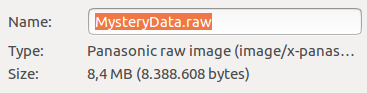
\includegraphics[width=0.6\textwidth]{res/file_size.png}
\caption{Size of MysteryData.raw}
\label{img:file_size}
\end{figure}

If the dimensions of a single image are $256x256$, there are 128 images $(8,388,608/(256x256))$; otherwise, if they are $512x512$, the number of images is 32 - since each dimension is doubled, the number is divided by 4. Both options are represented in Figure~\ref{img:settings}.
I selected “unsigned char” as Data Scalar Type because each pixel is represented using 1 byte.

\begin{figure}[htbp]
    \centering
	\begin{minipage}{0.45\textwidth}
        \centering
        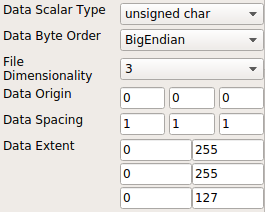
\includegraphics[width=0.9\textwidth]{res/settings_a.png} % first figure itself
    \end{minipage}\hfill
    \begin{minipage}{0.45\textwidth}
        \centering
        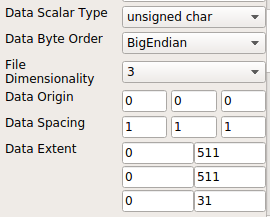
\includegraphics[width=0.9\textwidth]{res/settings_b.png} % second figure itself
	\end{minipage}
\caption{Different settings for ParaView.}
\label{img:settings}
\end{figure}

Using the Histogram filter (Figure~\ref{img:histogram}), we find two spikes in the distribution: one is place in the interval $[0, 25]$ and the second one in the interval $[50, 75]$.

\begin{figure}[htbp]
\centering
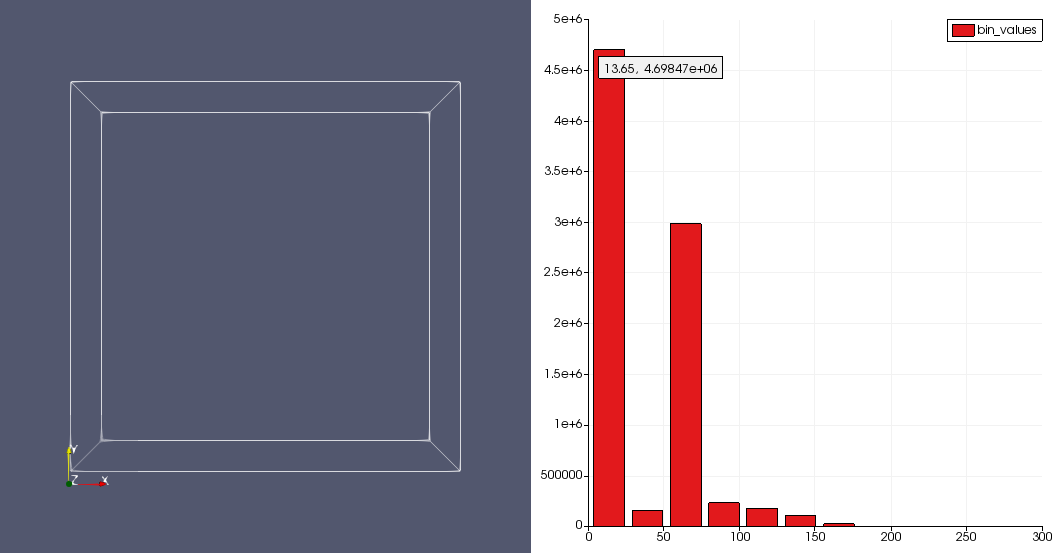
\includegraphics[width=0.9\textwidth]{res/screen_hist.png}
\caption{Result of histogram filter.}
\label{img:histogram}
\end{figure}

I added a Contour filter in order to visualize the Surface of the object (Isosurface value 25), but instead of a single one I obtained two object, so I changed the Data Extent matrix (Figure~\ref{img:data_extent}).

\begin{figure}[htbp]
\centering
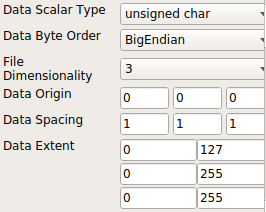
\includegraphics[width=0.45\textwidth]{res/data_extent.png}
\caption{Values assigned to the Data Extent matrix.}
\label{img:data_extent}
\end{figure}

\section{Results}

The result is a face of a person which is presumably covered in blood, as shown in Figure~\ref{img:face}.

\begin{figure}[htbp]
\centering
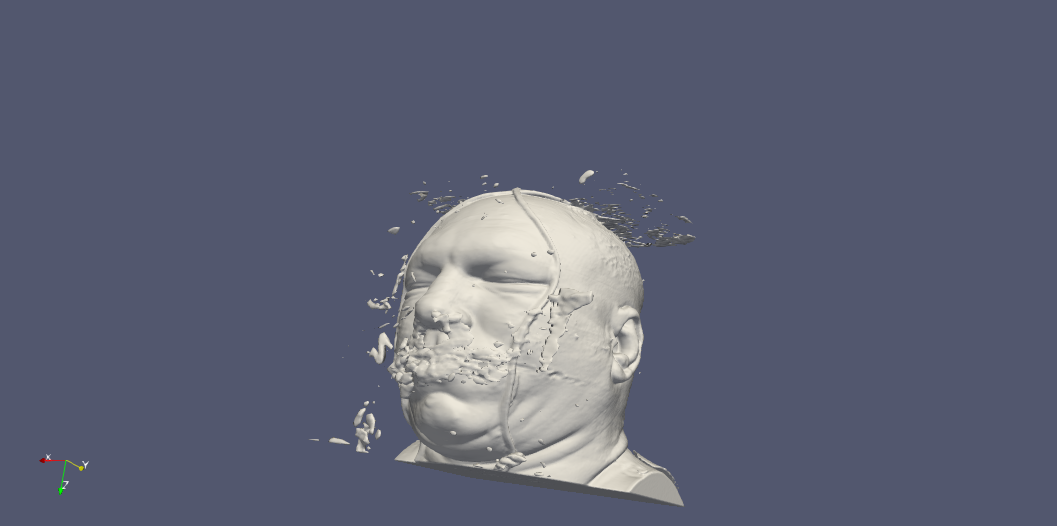
\includegraphics[width=0.8\textwidth]{res/face.png}
\caption{Result after the application of the Contour filter.}
\label{img:face}
\end{figure}

I added the remaining interval (i.e., [50, 75]) found thanks to the histogram and set opacity to 0.3. We can see that there are some strange stains between the skull and the skin, which could mean an intracranical effusion (Figure~\ref{img:face_opacity}). 

\begin{figure}[htbp]
\centering
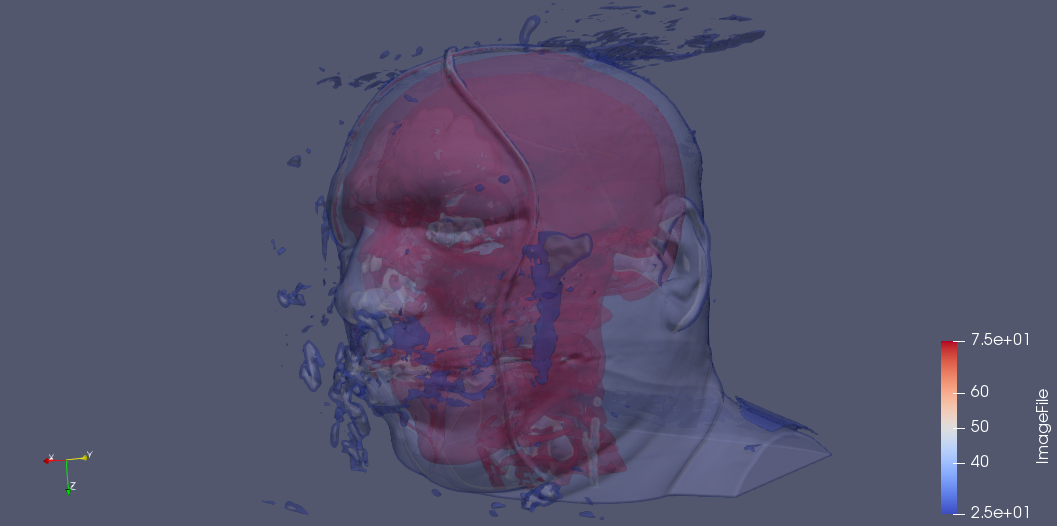
\includegraphics[width=0.8\textwidth]{res/opacity.png}
\caption{Result after the application of the Contour filters and Opacity.}
\label{img:face_opacity}
\end{figure}

In order to understand better what happened, I removed the previous values for the Isosurface, keeping only 75 as value. The result is shown in Figure~\ref{img:skull}.

\begin{figure}[htbp]
\centering
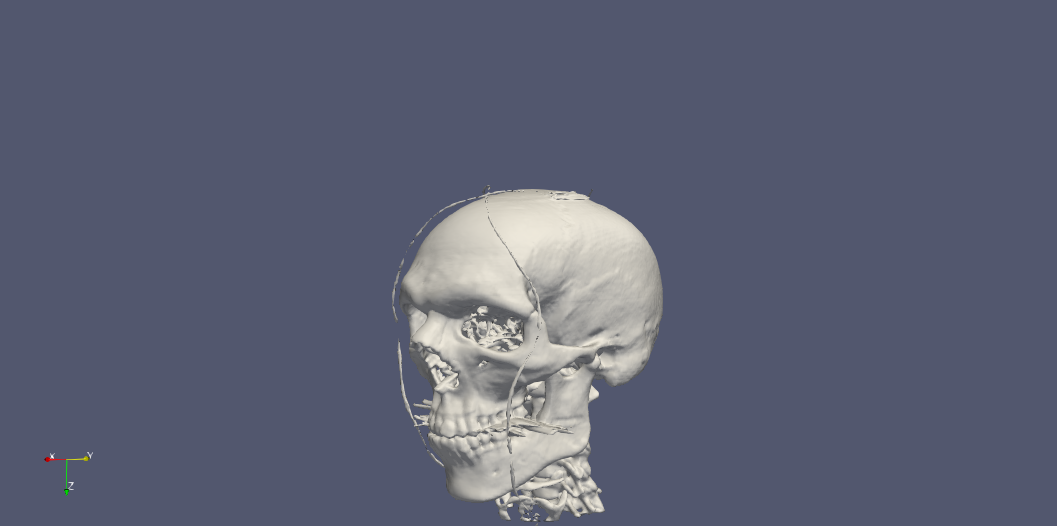
\includegraphics[width=0.8\textwidth]{res/skull.png}
\caption{Result after the application of the Contour filter with 75 as value.}
\label{img:skull}
\end{figure}

We can see that there is something like needles in the mouth of this person. If we rotate the image, we can also see that his jaw is broken (Figure~\ref{img:broken}).

\begin{figure}[htbp]
\centering
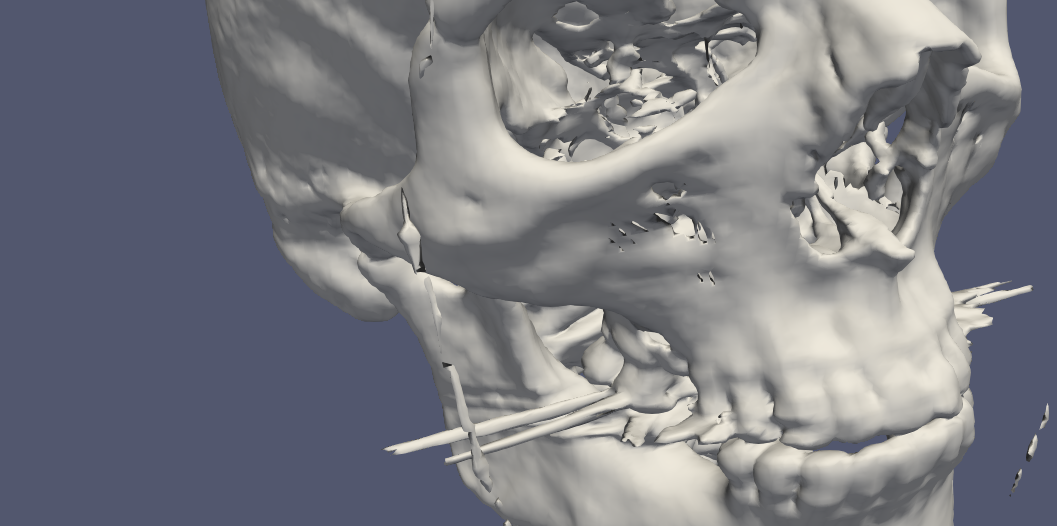
\includegraphics[width=0.8\textwidth]{res/broken.png}
\caption{Detail of the broken jaw.}
\label{img:broken}
\end{figure}

In fact, if we check better the initial image we can see that the tips of the needles and also a lot of blood coming out from his mouth in Figure~\ref{img:detail}.

\begin{figure}[htbp]
\centering
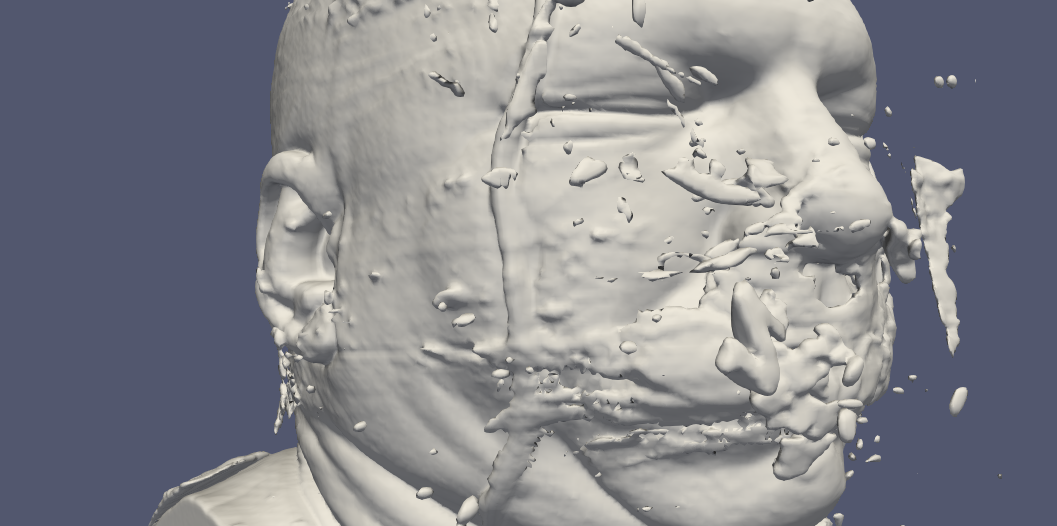
\includegraphics[width=0.8\textwidth]{res/detail.png}
\caption{Detail of the skull.}
\label{img:detail}
\end{figure}

The most likely hypothesis is that this person has been assassinated using those needles, thus loosing a lot of blood from his mouth. However, it is not clear where the two blood streams on his head are coming from, since I did not found any other abnormality.

\end{document}
